\documentclass{beamer}

\usetheme{simple}

\usepackage{lmodern}
\usepackage[utf8]{inputenc}
\usepackage{graphicx}
\usepackage{hyperref}
\usepackage{listings}
\usepackage[scale=2]{ccicons}

% TODO: 
%   position adjustement
%   change colours
%       

% Watermark background (simple theme)

\setwatermark{
\includegraphics[height=8cm]{img/docker.png}}


\title{VIRT - Treinamento da Plataforma de Virtualizacao Xen/Docker}
\subtitle{}
\date{\today}
\author{Agnaldo N. Marinho \\ Gabriel Silva}
\institute{\url{http://github.com/agnaldom}}

\begin{document}

\maketitle

\begin{frame}{Docker}
  \framesubtitle{Introdu\c{c}\~ao ao docker}

  \texttt{Docker} \'e uma plataforma aberta, criada com o objetivo de facilitar o desenvolvimento, 
  a implata\c{c}\~ao e a execu\c{c}\~ao de aplica\c{c}\~oes em ambientes isolados. 

  Usando o Docker, voc\^e pode facilmente gerenciar a infraestrutura da aplica\c{c}\~ao, isso agilizar\'a 
  o processo de cria\c{c}\~ao, manuten\c{c}\~ao e modifica\c{c}\~ao do seu servi\c{c}o.
\end{frame}

\begin{frame}{Docker}
    \framesubtitle{Container vs Virtual machines}
    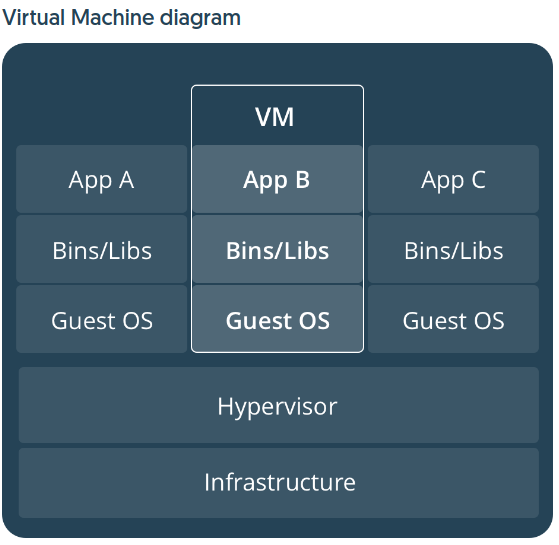
\includegraphics[height=5.7cm]{img/vm.png}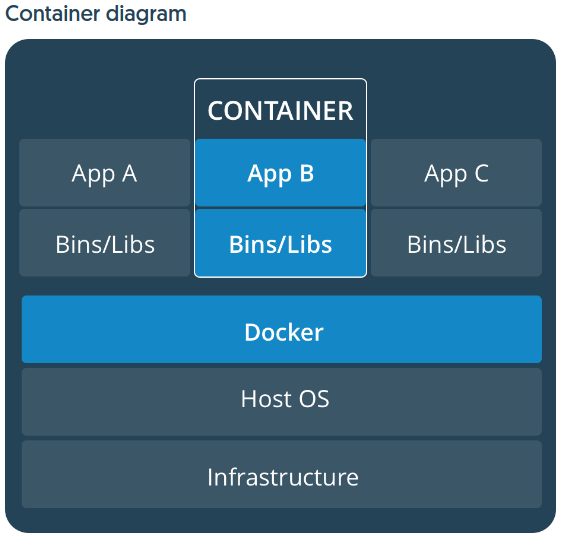
\includegraphics[width=6cm]{img/container.png}
\end{frame}

\begin{frame}{Docker}
    \framesubtitle{Instala\c{c}\~ao Docker}
    \begin{itemize}
        \item Docker est\'a disponivel em duas edi\c{c}\~oes: Community Edition (CE) e Enterprise Edition (EE).
        \item Docker (CE) \'e ideial para desenvolvedores e pequena equipes.
        \item Docker (EE) \'e voltado para times de desenvolvimento e TI das empresas.
    \end{itemize}
    No nosso caso vamos usar o (CE), e para vers\~ao do \href{https://docs.docker.com/engine/installation/linux/docker-ce/debian/}{debian stretch}.
\end{frame}

\begin{frame}{Docker}
    \framesubtitle{Inciando o seu primeiro container}
    Depois da instala\c{c}\~ao, vamos testar a instala\c{c}\~ao rodando o seguinte:
    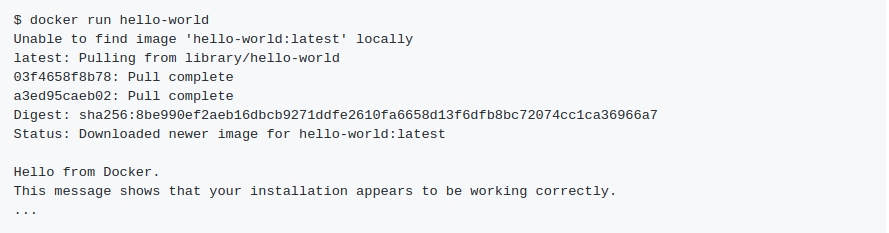
\includegraphics[height=5cm]{img/hello.png}
\end{frame}

\begin{frame}{Docker}
    \framesubtitle{Comandos básicos}
    Para iniciar um container \'e necess\'ario saber a partir de qual imagem será executado. Para lista as
    images que o seu Docker Host tem localmente, execute o comando abaixo>
    \begin{enumerate}
        \item  docker image list
    \end{enumerate}
    Baixando a imagem
    \begin{enumerate}
        \item docker image pull debian
    \end{enumerate}
    Baixamos uma imgem do debian, caso deseje inspecionar a imagem que acabou de atualizar, bastar usar o comando abaixo:
    \begin{enumerate}
        \item docker image inspect debian
    \end{enumerate}
    O comando inspect \'e respons\'avel por informa todos os dados referentes \`a imagem.
\end{frame}

\begin{frame}{Docker}
    \framesubtitle{Criando sua pr\'opria imagem no Docker}
    Uma imagem nada mais \'e do que um ambiente totalmente encapsulado e pronto para ser replicado onde desejar.
    Há duas formas de criar images customizadas: com commit e com Dockerfile.
    \begin{itemize}
        \item Criando images com commit
    \end{itemize}
    Primeiro criamos um container :
    \begin{enumerate}
        \item docker run -it --name dockercurso-debian debian:latest /bin/bash
    \end{enumerate} 
    Agora que estamos no bash do container, instalamos o nginx:
    \begin{enumerate}
        \item apt-get update
        \item apt-get install nginx -y
        \item exit
    \end{enumerate}
    Paramos o container com o comando abaixo:
    \begin{enumerate}
        \item docker container stop dockercurso-debian 
    \end{enumerate}
\end{frame}

\begin{frame}{Docker}
    \framesubtitle{Criando sua pr\'opria imagem no Docker}
    Agora, efetuamos o commit desse container em uma imagem:
    \begin{enumerate}
        \item docker container commit dockercurso-debian dockercurso-nginx
    \end{enumerate}
    Para visualizar a lista de imagens e encontrar a que acabou de criar,
    execute novamente o comando abaixo:
    \begin{enumerate}
        \item docker image list
    \end{enumerate}
    Para testar sua nova image, vamos criar um container a parti dela e verificar se o nginx está instalado:
    \begin{enumerate}
        \item docker run -it --rm dockercurso-nginx dpkg -l nginx
    \end{enumerate}
\end{frame}

\begin{frame}{Docker}
    \framesubtitle{Criando imagens com Dockerfile}
    O docker permite que possamos criar images a partir de um arquivo de defini\c{c}\~ao, 
    esse arquivo chama-se Dockerfile. Em resumo, o Dockerfile  um arquivo texto com
    instru\c{c}~oes, comandos e passos que voc\^e executaria manualmente, basicamente
    o Docker executa uma receita de bolo.
    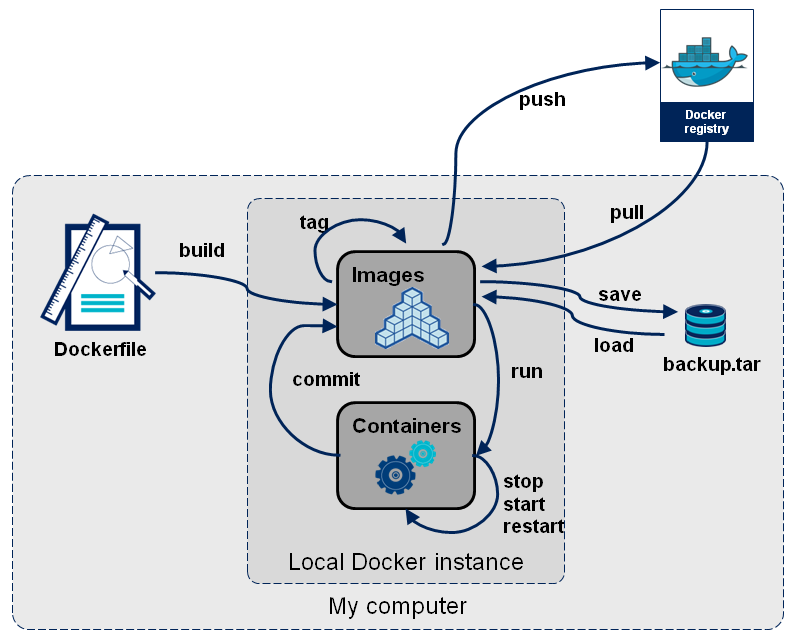
\includegraphics[height=5cm]{img/docker-stages.png}
\end{frame}

\begin{frame}{Docker}
    \framesubtitle{Criando imagens com Dockerfile}
    Atrav\'es do comando docker build, o Docker realizar a execu\c{c}\~ao desses passos 
    e no fina da execu\c{c}\~ao ele encapsula cada layer gerada dentro da imagem.

    O Dockerfile deve seguir uma ordem ou formata\c{c}\~ao correta para que o build
    seja feito de forma certa.

    Exemplo:

    RUN apt-get update

    onde:

    RUN  \'E a instru\c{c}\~ao;

    apt-get update: Argumento que ser\'a executado.

    \href{https://docs.docker.com/engine/reference/builder/}{Dockerfile Referência Oficial}
\end{frame}


\begin{frame}{Docker}
    \framesubtitle{Criando imagens com Dockerfile}
    \href{https://github.com/agnaldom/curso-docker/blob/master/images/nginx/Dockerfile}{
\includegraphics[height=5cm]{img/docker-nginx.png}}
\end{frame}
\begin{frame}{Docker}
    \framesubtitle{Criando imagens com Dockerfile}
    
\includegraphics[height=2cm]{img/docker-php.png}
\end{frame}
\begin{frame}{Docker}
  \framesubtitle{Teste}
  \begin{columns}
    \column{.5\textwidth}
      \begin{itemize}
        \item a \alert{watermark} logo in the background
        \item slide \alert{numbers}
        \item \emph{emph}asized and \alert{alert}ed text
      \end{itemize}

    \column{.5\textwidth}
      \begin{block}{And of course...}
         blocks, columns, and all Beamer power
      \end{block}
  \end{columns}
\end{frame}



\setwatermark{\fontsize{125pt}{125pt}\selectfont{Simple}}

\begin{frame}[fragile]{watermark}
  \framesubtitle{not only for images}

  \begin{itemize}
    \item You can place \emph{any} \LaTeX{} \alert{contents} as a watermark
  \end{itemize}

  \begin{block}{In preamble}
    \begin{verbatim}
     \setwatermark{
\includegraphics[height=8cm]{%
                   img/Heckert_GNU_white.png}}
    \end{verbatim}
  \end{block}

  \begin{block}{Just before this frame}
    \begin{verbatim}
     \setwatermark{\fontsize{125pt}{125pt}%
                   \selectfont{Simple}}
    \end{verbatim}
  \end{block}


\end{frame}



\setwatermark[hoffset=-3cm,voffset=-2cm]{\fontsize{125pt}{125pt}\selectfont{Simple}}


\begin{frame}{Options}
  \framesubtitle{Fine adjustement of the watermark position}

  
  \begin{itemize}
    \item \texttt{hoffset}
    \item \texttt{voffset}
  \end{itemize}
  
  They admit any \emph{positive} or \emph{negative} spacing \alert{unit}
  
  Note that some \alert{warnings} about \emph{badboxes} might be generated at compilation

\end{frame}




\begin{frame}{License}

  \begin{block}{Get the source of this theme and the demo presentation from}

  \begin{center}\url{http://github.com/famuvie/beamerthemesimple}\end{center}

  \end{block}
  
  The theme \emph{itself} is licensed under a
  \href{http://creativecommons.org/licenses/by-sa/4.0/}{Creative Commons
  Attribution-ShareAlike 4.0 International License}.

  \begin{center}\ccbysa\end{center}

\end{frame}

\end{document}

